%% Healthy Lifestyle RL --- Capstone Report (V3)
%% EECS 590 Reinforcement Learning, Spring 2026
%% IEEE conference format (IEEEtran).
\documentclass[conference]{IEEEtran}
\IEEEoverridecommandlockouts

\usepackage{cite}
\usepackage{amsmath,amssymb,amsfonts}
\usepackage{graphicx}
\usepackage{booktabs}
\usepackage{array}
\usepackage{textcomp}
\usepackage{xcolor}
\usepackage[hidelinks]{hyperref}
\usepackage{url}

% Professional academic color palette (navy + slate). No pink.
\definecolor{navy}{RGB}{11,61,89}
\definecolor{slate}{RGB}{70,90,105}
\hypersetup{
  colorlinks=true,
  linkcolor=navy,
  citecolor=navy,
  urlcolor=navy
}

% Inline-code style without garish colors.
\newcommand{\code}[1]{\texttt{\small #1}}

% Keep figures from floating too far; discourage ugly page-splitting.
\renewcommand{\topfraction}{0.9}
\renewcommand{\bottomfraction}{0.8}
\renewcommand{\textfraction}{0.07}
\renewcommand{\floatpagefraction}{0.7}

\graphicspath{{../results/plots/}}

\begin{document}

\title{Healthy Lifestyle RL: Safe Deep Reinforcement\\
Learning for Personalized Nutrition, Sleep,\\
and Activity Recommendation}

\author{
\IEEEauthorblockN{Ismail Gargouri}
\IEEEauthorblockA{
Department of Computer Science\\
University of North Dakota\\
EECS 590 --- Reinforcement Learning, Spring 2026\\
ismail.gargouri@und.edu}
}

\maketitle

\begin{abstract}
This capstone investigates whether a single reinforcement-learning (RL)
agent, trained on a custom Gymnasium-compatible simulator, can outperform
two non-learning baselines---uniform random and a fitness-planner
heuristic---at recommending small daily adjustments to a simulated user's
calorie, sleep, step, and protein targets across a 60-day horizon. The agent
is constrained by a configurable \emph{safety layer} that clips unsafe action
proposals before they reach the transition model, and is trained against a
reward decomposition that explicitly penalizes unsafe proposals, rapid daily
changes, and weight-trajectory instability. Two algorithms are implemented: a
Deep Q-Network (DQN) written from scratch in PyTorch, and a Proximal Policy
Optimization (PPO) agent built on Stable-Baselines3. Bayesian (Tree-structured
Parzen Estimator) hyperparameter search is applied to the DQN agent. All four
policies are evaluated across five simulated user profiles. We report a
concrete case of reward hacking under a safety constraint, and document the
methods deliberately \emph{not} implemented (multi-agent, swarm, robotics
simulators, offline RL, Sim2Real, meta-RL, hierarchical RL) with explicit
justification.
\end{abstract}

\begin{IEEEkeywords}
reinforcement learning, Markov decision process, deep Q-network, proximal
policy optimization, safe RL, hyperparameter optimization.
\end{IEEEkeywords}

\section{Introduction}
A user trying to maintain a healthy lifestyle makes dozens of small decisions
every day: how much to eat, when to sleep, when to push activity, and when to
rest. Most of these choices are fine in isolation but couple in ways that are
hard to see ahead of time. Pushing activity hard on a low-sleep day degrades
recovery, which degrades next-day adherence, which in turn degrades next-week
consistency. The effect of today's choices surfaces days later in recovery and
weight-trend signals. This temporal structure is precisely what makes the
problem interesting from an RL perspective: it is a sequential decision problem
with delayed reward \cite{sutton}, and exactly the kind of problem a competent
rule-based planner can approximate but only an agent with credit assignment can
learn end to end.

The goal of this capstone is not to \emph{deploy} such an agent---the safety
and validation requirements for real-world health recommendation are well
outside what belongs in a semester project---but to build the simulator, the
safety layer, the agents, and the evaluation harness that would form the
starting point for a more serious effort. All code, configurations, metrics,
and plots are released as an open-source repository.

\section{Problem Formulation}
We model one day in the user's life as one step in a Markov decision process
(MDP) $(\mathcal{S}, \mathcal{A}, P, R, \gamma)$ \cite{sutton}. The agent
observes a normalized 18-dimensional summary of the user's static profile and
dynamic state, selects one of eight discrete adjustment actions, the safety
layer translates that action into per-day target deltas and clips them, and the
transition model rolls forward one simulated day. The reward is a weighted sum
of eight components.

The single-agent framing is deliberate. The unit of optimization is
\emph{one} user, not a group or a fleet, which rules out multi-agent and
coordination methods. Table~\ref{tab:mdp} summarizes the MDP.

\begin{table}[!t]
\renewcommand{\arraystretch}{1.25}
\caption{MDP Specification}
\label{tab:mdp}
\centering
\footnotesize
\begin{tabular}{@{}p{1.4cm}p{6.0cm}@{}}
\toprule
\textbf{Component} & \textbf{Definition} \\
\midrule
States &
18-dim normalized vector: age, sex, height, initial weight, goal-type code,
current weight, 7-day weight trend, calorie target, actual intake,
protein/carbs/fat, sleep hours, steps, recovery, adherence, energy, and
normalized day index. Box$(-2,2)^{18}$. \\
Actions &
8 discrete adjustments: maintain, decrease/increase calories, increase
activity, prioritize recovery, increase sleep, raise protein, rebalance carbs.
Discrete(8). \\
Transition &
Stochastic; adherence-weighted realization of targets, recovery driven by sleep
and load, slow weight evolution via the 7700~kcal/kg energy-balance
approximation. \\
Reward &
Eight weighted components (Section~\ref{sec:reward}). \\
Horizon &
60 days (configurable: 30/60/90). \\
Discount &
$\gamma = 0.99$. \\
\bottomrule
\end{tabular}
\end{table}

\section{Environment Design}
\code{HealthyLifestyleEnv} implements the standard \code{reset}~$\rightarrow$
\code{step} Gymnasium API \cite{gymnasium} and a text \code{render}. Each
\code{step()} returns the standard five-tuple
$(\mathit{obs}, r, \mathit{terminated}, \mathit{truncated}, \mathit{info})$ plus
an \code{info} dictionary exposing the raw action, the safe action, whether a
safety intervention was applied, the clipped components, the action's
natural-language meaning, current weight, weight trend, adherence/recovery/energy
scores, calorie target, sleep hours, steps, and the per-component reward
breakdown. Surfacing every quantity in \code{info} made debugging far easier:
when a training curve looked wrong, a single inspection of
\code{info["reward\_components"]} revealed which component was misbehaving.

Profiles are drawn from a library of five personas (\code{maintenance},
\code{general\_wellness}, \code{activity\_consistency},
\code{gradual\_management}, \code{performance\_support}) and optionally jittered
with Gaussian noise on age, height, and weight. The jitter is reproducible---it
is driven by the environment's seeded RNG---so rollouts are repeatable.

\section{Reward Decomposition}
\label{sec:reward}
The per-step reward combines five positive and three negative terms:
\begin{align}
r =\ & w_{\text{goal}}\, g(\text{state},\text{profile})
      + w_{\text{adh}}\, a
      + w_{\text{sleep}}\, b(\text{sleep}) \nonumber\\
   & + w_{\text{act}}\, b(\text{steps})
      + w_{\text{rec}}\, c \nonumber\\
   & - w_{\text{unsafe}}\, u
      - w_{\text{rapid}}\, \Delta
      - w_{\text{stab}}\, s,
\end{align}
where $a$ is the adherence score, $c$ the recovery score, $u$ the unsafe-proposal
indicator, $\Delta$ the total absolute target movement, and $s$ the per-day
weight swing. The function $b(\cdot)$ returns 1.0 inside a target window and
decays as a Gaussian outside it.

Getting the penalty signs right mattered early: the first version contained
$+w_{\text{unsafe}}\,u$, which \emph{rewarded} the agent for triggering safety
interventions. The bug was caught by a unit test rather than by inspection, and
it is the main reason \code{test\_rewards.py} includes an explicit
unsafe-penalty test. All weights live in \code{configs/env.yaml} and are
configurable for ablation.

\section{Safety Layer}
The safety layer is the most architecturally important piece of the project. It
sits \emph{between} the agent and the simulator: the agent emits an action id,
the layer maps it to per-day deltas, clips those deltas against configurable
bounds, and reports the intervention back through \code{info}. The bounds are
listed in Table~\ref{tab:safety}.

\begin{table}[!t]
\renewcommand{\arraystretch}{1.2}
\caption{Configurable Safety Constraints}
\label{tab:safety}
\centering
\footnotesize
\begin{tabular}{@{}lll@{}}
\toprule
\textbf{Constraint} & \textbf{Default} & \textbf{Prevents} \\
\midrule
min calorie target        & 1500 kcal   & extreme restriction \\
max calorie target        & 3500 kcal   & extreme surplus \\
max daily calorie change  & 150 kcal    & large single-day swings \\
min sleep target          & 6.5 h       & sleep deprivation \\
max sleep target          & 9.5 h       & pathological oversleeping \\
max step increase/day     & 1500 steps  & sudden activity spike \\
min recovery threshold    & 0.35        & training under-recovered \\
min protein               & 1.2 g/kg    & protein deficiency \\
max protein               & 2.4 g/kg    & excessive protein \\
\bottomrule
\end{tabular}
\end{table}

A separate low-recovery override forces a recovery action when the recovery
score falls below the threshold, regardless of the agent's choice. Every
intervention is surfaced in the reward as an unsafe-action penalty, so the layer
acts simultaneously as a hard constraint (clipping) and a soft constraint
(penalty), giving the agent a learning signal to stay inside the safe envelope
voluntarily.

\section{Algorithms}
\subsection{Random and rule-based baselines}
The random policy samples uniformly from the action space. The rule-based policy
is a deterministic heuristic: if adherence is low, maintain; if recovery is low,
recover; if sleep is low, sleep; if the 7-day weight trend is outside the goal
window, nudge calories. Both set the floor the RL agents must beat. The
heuristic is a deliberately strong competitor, which is a useful calibration
rather than a problem.

\subsection{DQN (custom PyTorch)}
DQN \cite{dqn-nature,dqn-atari} was implemented first because the course derived
the Q-learning update in detail and the implementation mirrors that derivation.
All core ideas from \cite{dqn-nature} are present: a 50k-transition experience
replay buffer that decorrelates consecutive samples; a target network held fixed
for \code{target\_update\_freq} steps to stabilize the Bellman target
$r + \gamma \max_{a'} Q_{\text{target}}(s',a')$; $\epsilon$-greedy exploration
decaying linearly from 1.0 to 0.05; Huber (smooth-$L_1$) loss for robustness to
large temporal-difference errors; and gradient clipping at norm 10. The
Q-network is a two-hidden-layer MLP ($128 \rightarrow 128 \rightarrow 8$).

\subsection{PPO (Stable-Baselines3)}
PPO \cite{ppo} uses a clipped surrogate objective to bound each policy update,
making it more stable than vanilla policy gradient. We use Stable-Baselines3
\cite{sb3} rather than a hand-rolled PPO because PPO has several
correctness-sensitive components---the clipped surrogate, generalized advantage
estimation \cite{gae}, the value-loss coefficient, and the entropy bonus---that
are easy to get subtly wrong. Writing one carefully derived algorithm from
scratch (DQN) and using one well-tested library implementation (PPO) yields a
more honest project than two half-correct custom rolls. PPO is configured with
\code{n\_steps=512}, \code{ent\_coef=0.01}, and \code{clip\_range=0.2}.

\subsection{Bayesian hyperparameter tuning}
\code{tune\_bayesian.py} uses Optuna's TPE sampler \cite{optuna} to search over
$\{\text{learning rate}, \gamma, \text{batch size}, \text{hidden size},
\epsilon\text{-decay}\}$ on the DQN agent, maximizing mean episode reward over
the trailing 20\% of training. Bayesian search matters here: a 5-parameter grid
with 4--5 values each is 1024--3125 trials, prohibitive when each trial takes
tens of seconds. TPE concentrates its budget where the surrogate predicts the
next trial is most informative \cite{optuna}.

\section{Experiments and Results}
Each policy is evaluated for 20 episodes per profile across all five profiles
(100 rollouts per policy, 400 total). Metrics: mean episode reward, mean
safety-intervention rate, mean adherence, mean recovery, and action-frequency
distribution. Aggregate results appear in Table~\ref{tab:agg} and per-profile
rewards in Table~\ref{tab:perprofile}.

\begin{table}[!t]
\renewcommand{\arraystretch}{1.2}
\caption{Aggregate Results Across All Profiles}
\label{tab:agg}
\centering
\footnotesize
\begin{tabular}{@{}lcc@{}}
\toprule
\textbf{Policy} & \textbf{Mean reward} & \textbf{Interventions/ep} \\
\midrule
Random              & $\approx$178 & $\approx$3.6 \\
Rule-based          & $\approx$207 & $\approx$0.0 \\
DQN (250 ep)        & $\approx$198 & $\approx$0.1 \\
PPO (SB3)           & $\approx$202\textsuperscript{*} & $\approx$6.1\textsuperscript{*} \\
\bottomrule
\end{tabular}
\\[2pt]
\raggedright\textsuperscript{*}\,Skewed by the \code{gradual\_management}
anomaly (Section~\ref{sec:hacking}).
\end{table}

\begin{table}[!t]
\renewcommand{\arraystretch}{1.2}
\caption{Per-Profile Mean Reward}
\label{tab:perprofile}
\centering
\footnotesize
\begin{tabular}{@{}lcccc@{}}
\toprule
\textbf{Profile} & \textbf{Rand.} & \textbf{Rule} & \textbf{DQN} & \textbf{PPO} \\
\midrule
maintenance          & 177 & 206 & \textbf{202} & 205 \\
general\_wellness    & 181 & 208 & 197 & 197 \\
activity\_consist.   & 182 & 207 & 192 & \textbf{208} \\
gradual\_manage.     & 175 & 208 & 197 & 200 \\
performance\_supp.   & 175 & 208 & \textbf{203} & 201 \\
\bottomrule
\end{tabular}
\end{table}

\subsection{Baselines and learned agents}
The rule-based heuristic consistently scores 205--208 with zero safety
interventions on every profile---the ceiling the RL agents must approach. It is
not a trivial baseline: the heuristic was designed with full knowledge of the
reward components, while the RL agents must discover an effective policy from the
scalar reward alone.

The DQN used for final evaluation was trained for 250 episodes and reaches
192--203 depending on profile (Fig.~\ref{fig:dqncurve}). Training a 500-episode
variant did not close the gap: reward plateaus after episode 200 once
exploration ends, confirming convergence to a local optimum roughly 8--10 reward
points below the rule-based ceiling. Simply training longer does not help, which
partly motivates the tuning study (Fig.~\ref{fig:tuning}).

\begin{figure}[!t]
\centering
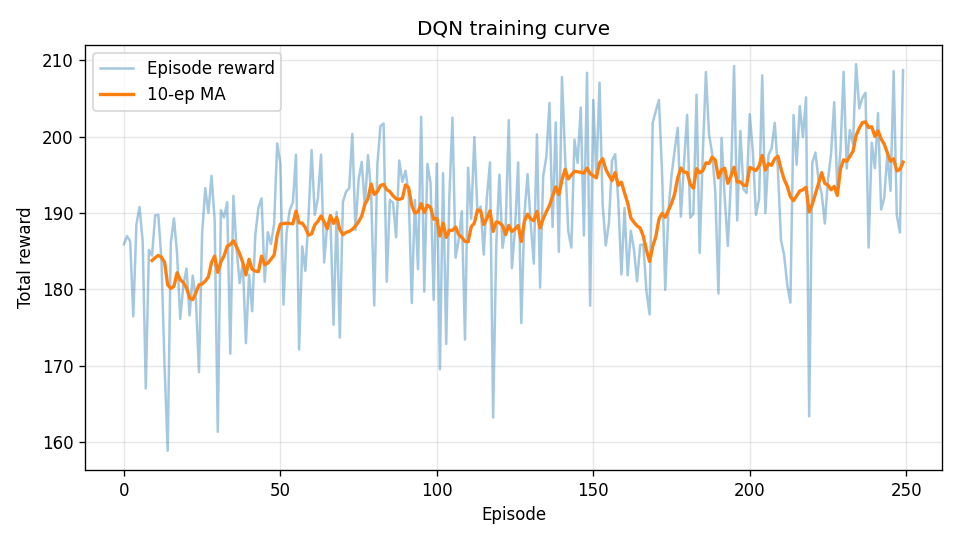
\includegraphics[width=\columnwidth]{dqn_training_curve.png}
\caption{DQN training curve (250 episodes). Reward climbs until exploration
ends near episode 200, then plateaus.}
\label{fig:dqncurve}
\end{figure}

\begin{figure}[!t]
\centering
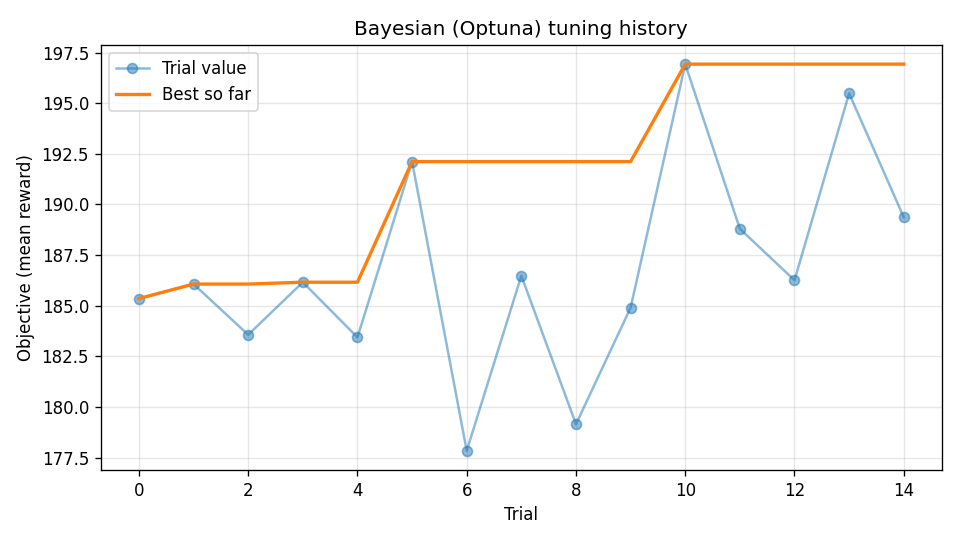
\includegraphics[width=\columnwidth]{tuning_history.png}
\caption{Optuna (TPE) tuning history for DQN. The best-so-far curve rises as the
sampler concentrates trials in the profitable region.}
\label{fig:tuning}
\end{figure}

Figs.~\ref{fig:reward}--\ref{fig:adherence} compare mean reward, safety
intervention counts, and adherence across policies; Fig.~\ref{fig:actions}
(spanning both columns) shows the action-frequency distribution.

\begin{figure}[!t]
\centering
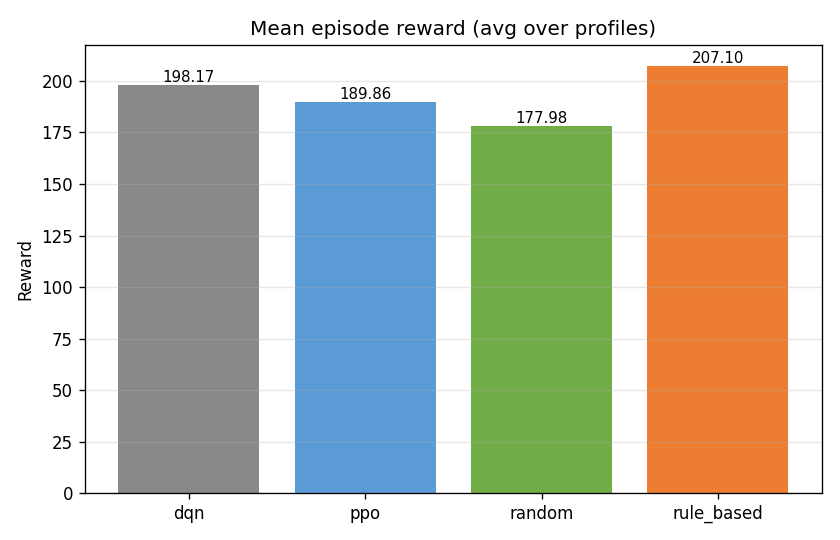
\includegraphics[width=\columnwidth]{reward_comparison.png}
\caption{Mean episode reward by policy.}
\label{fig:reward}
\end{figure}

\begin{figure}[!t]
\centering
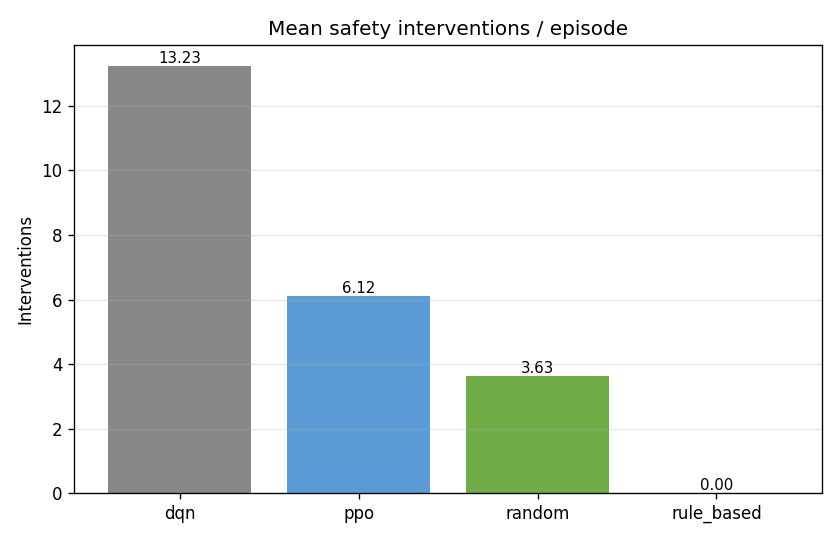
\includegraphics[width=\columnwidth]{safety_intervention_comparison.png}
\caption{Mean safety interventions per episode by policy. The random policy
exercises the safety layer; rule-based and DQN rarely trip it.}
\label{fig:safety}
\end{figure}

\begin{figure}[!t]
\centering
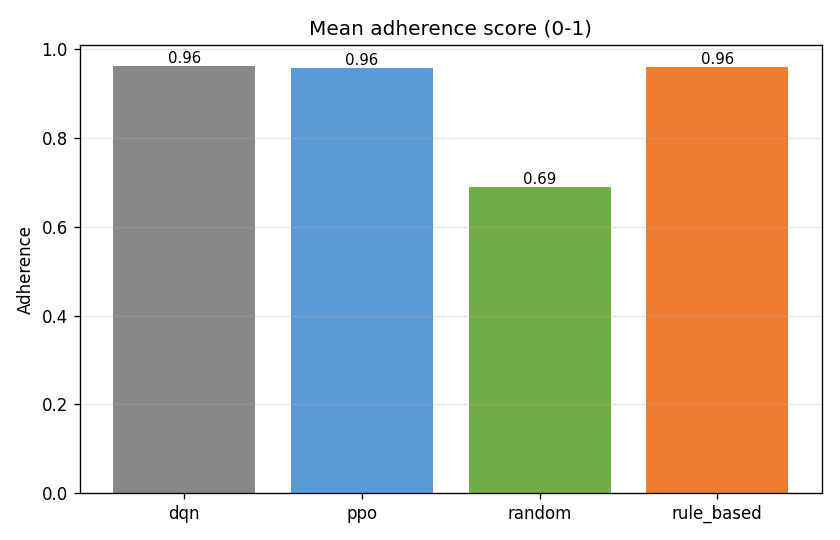
\includegraphics[width=\columnwidth]{adherence_comparison.png}
\caption{Mean adherence score by policy.}
\label{fig:adherence}
\end{figure}

\begin{figure*}[!t]
\centering
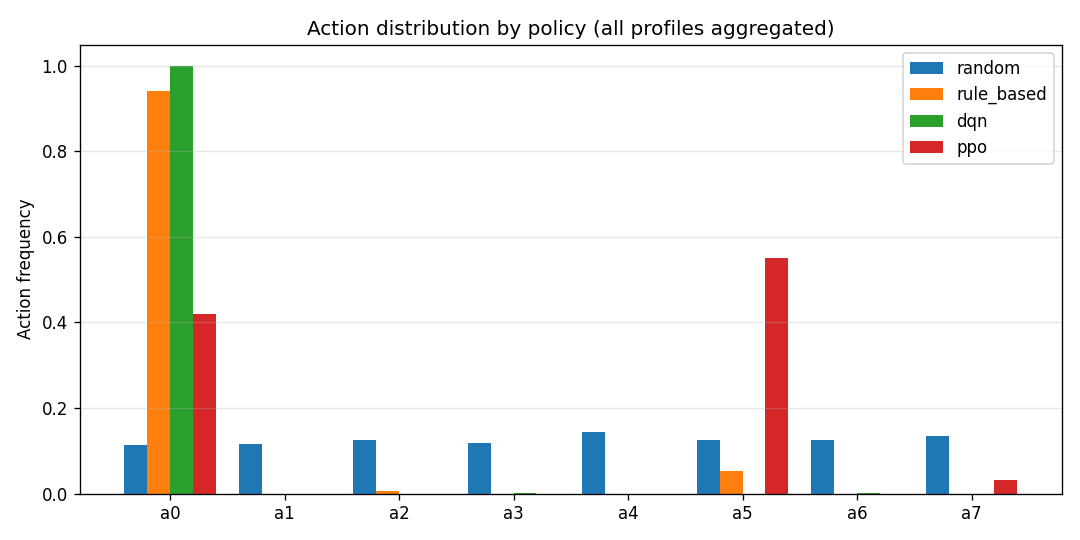
\includegraphics[width=0.92\textwidth]{action_distribution.png}
\caption{Per-action frequency grouped by policy. DQN and rule-based concentrate
on the ``maintain'' action; PPO spreads its mass across many actions.}
\label{fig:actions}
\end{figure*}

\subsection{Reward hacking under a safety constraint}
\label{sec:hacking}
PPO matches or beats DQN on most profiles but triggers a pathological number of
safety interventions on \code{gradual\_management} (30.4 per episode versus
$\approx$0 elsewhere). Per-episode inspection
(Fig.~\ref{fig:inspect}) makes the cause clear across three seeds: PPO
repeatedly proposes calorie-increase actions that the safety layer clips, ending
with the simulated user \emph{gaining} weight despite a slow-weight-loss goal,
while still earning high adherence and recovery reward. This is reward hacking:
from the policy's perspective the behavior looks good, but the goal is never met.
By contrast, DQN and the rule-based heuristic converge to nearly identical
trajectories---the same final weight ($\approx$80.5~kg), the same $-0.16$~kg/week
trend, and zero clips---confirming that DQN effectively rediscovered the
heuristic.

\begin{figure}[!t]
\centering
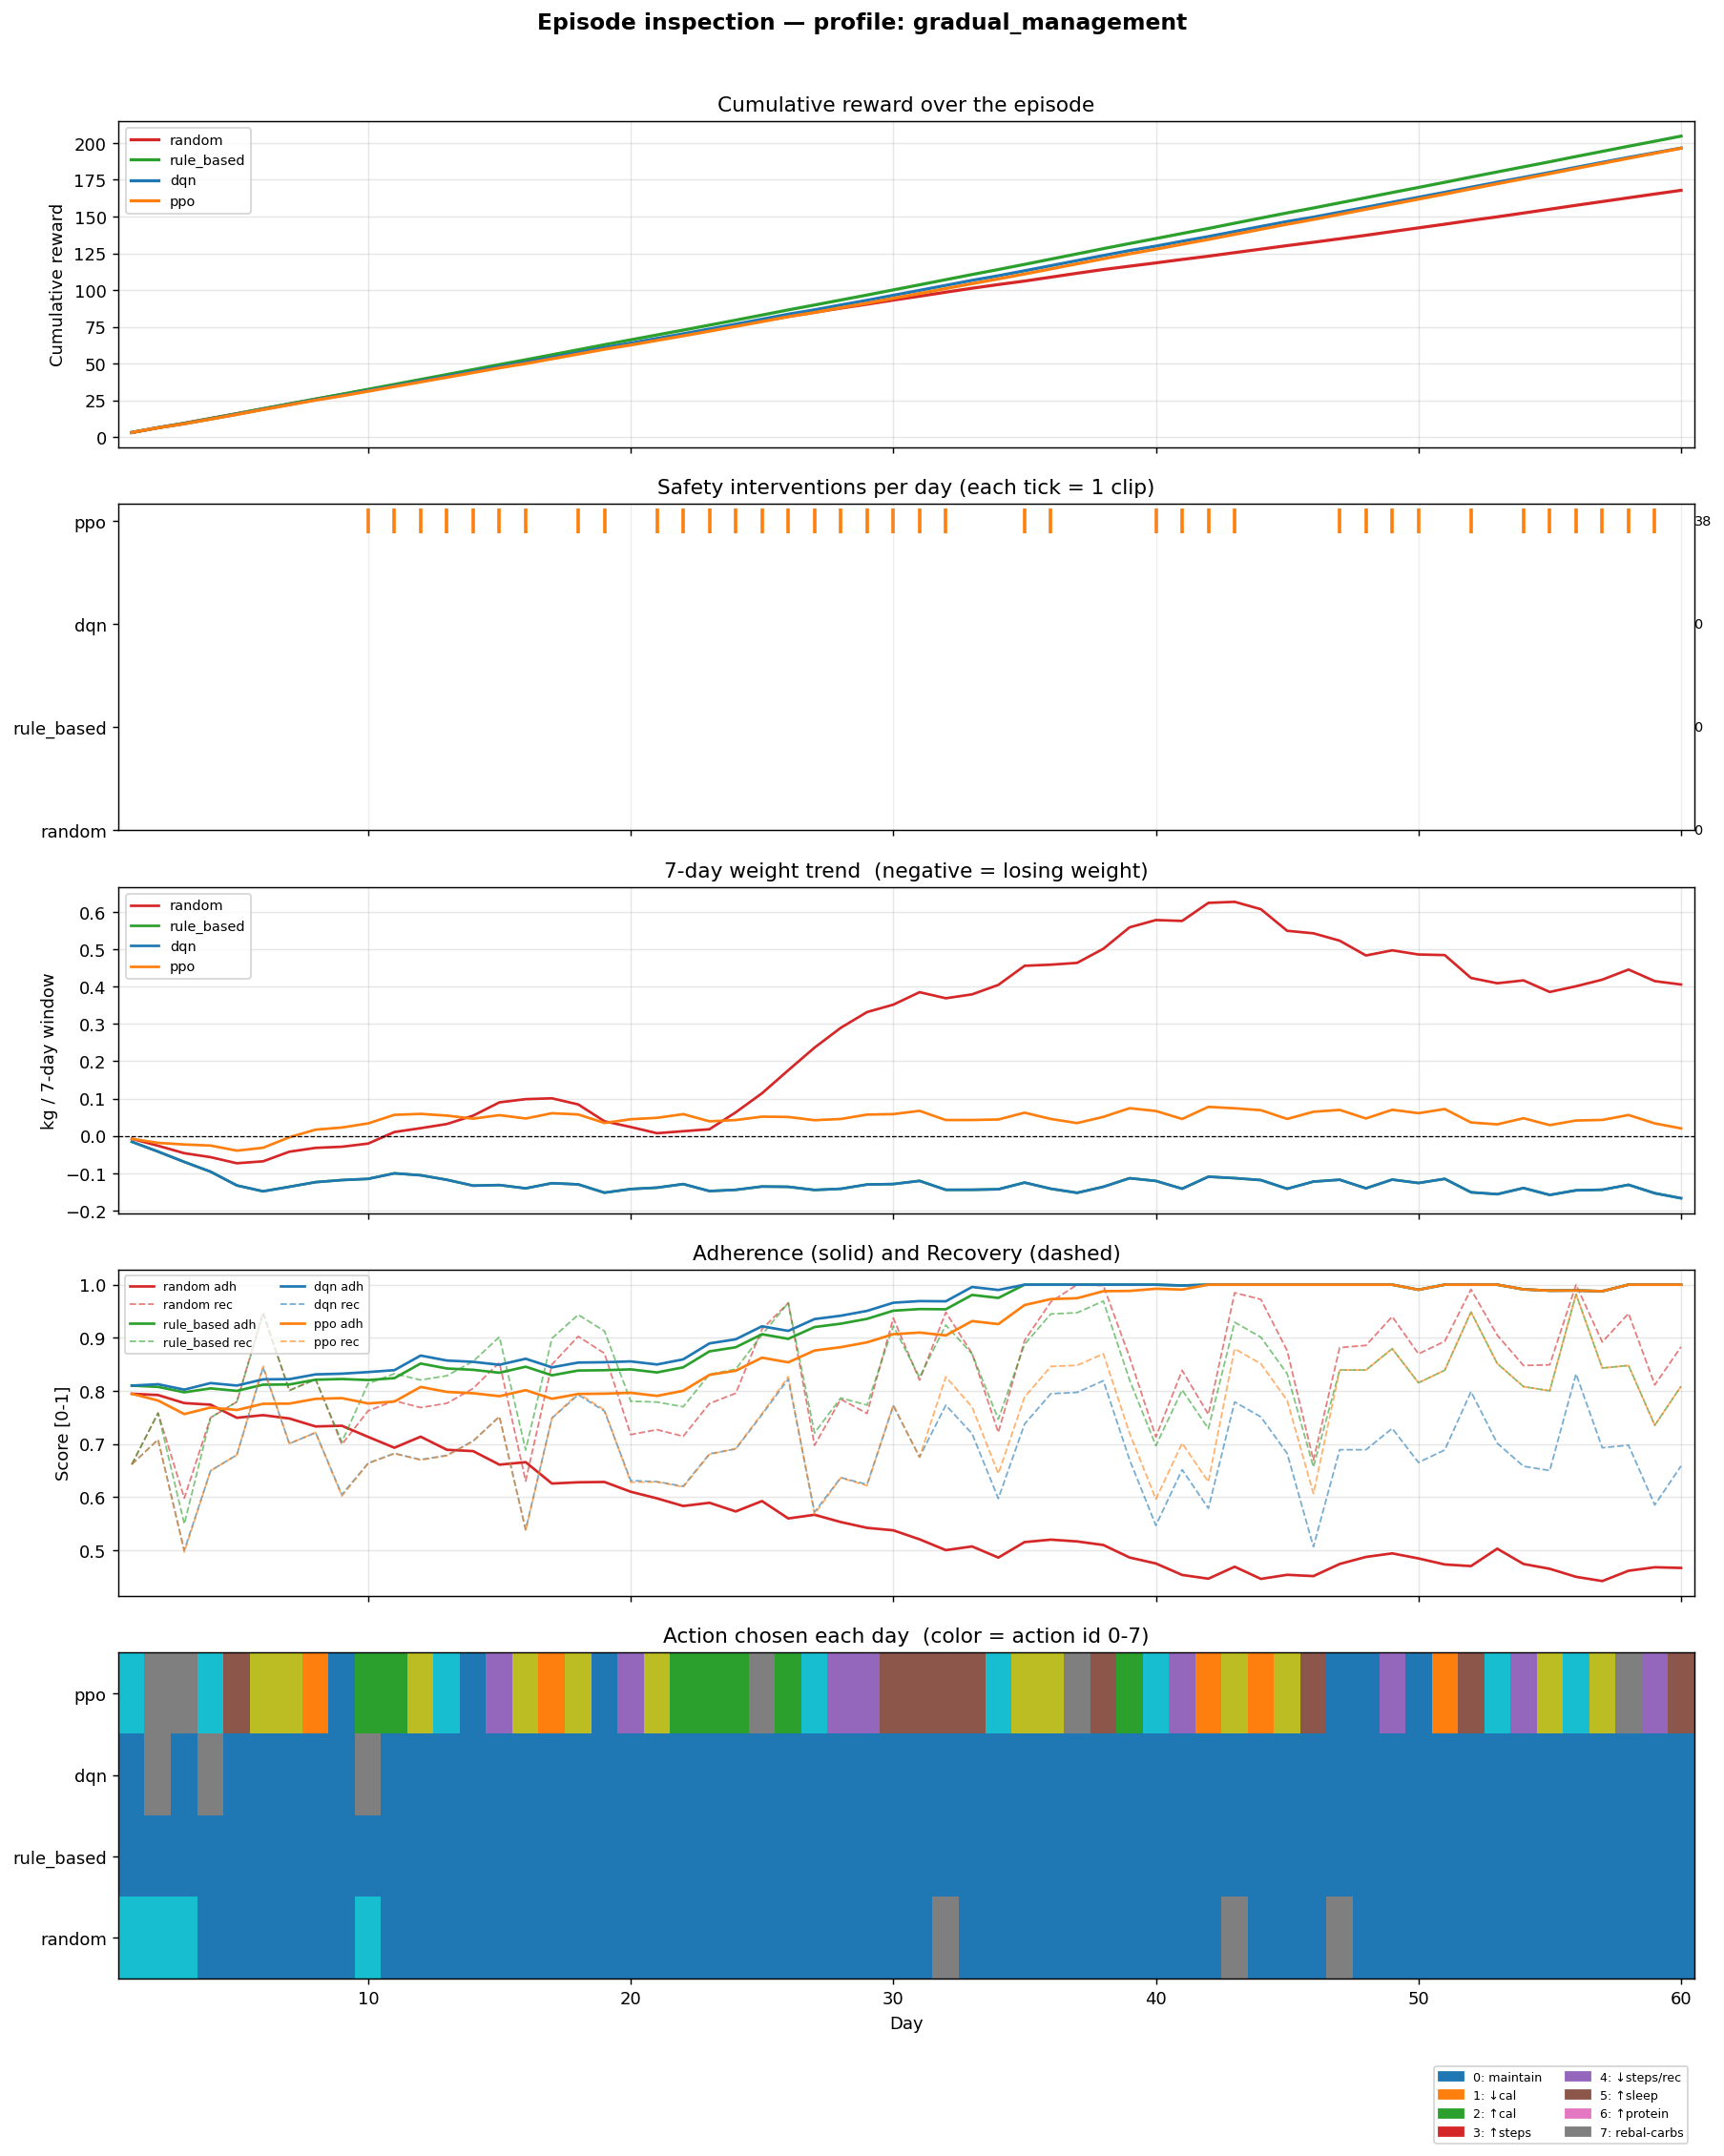
\includegraphics[width=\columnwidth]{inspect_gradual_management_ep7.png}
\caption{Single-episode inspection on \code{gradual\_management} (seed 7). Top to
bottom: cumulative reward, per-day safety-intervention raster, 7-day weight
trend, adherence (solid) and recovery (dashed), and the action chosen each day.
PPO's intervention stream and unstable weight trend are visible against DQN's
near-constant ``maintain'' policy.}
\label{fig:inspect}
\end{figure}

\subsection{A falsified hypothesis: high-entropy PPO}
To test whether more exploration would fix the anomaly, PPO was retrained with
\code{ent\_coef=0.05}. The result was unambiguously worse
(Table~\ref{tab:highent}): interventions on \code{gradual\_management} rose from
30.4 to 45.0 per episode, and previously clean profiles spiked sharply. Higher
entropy made the policy more erratic everywhere rather than more goal-aware. This
falsifies the exploration hypothesis and points instead to reward weighting: the
goal-progress term is not consequential enough relative to adherence and
recovery to motivate a calorie-reduction strategy. The principled fix is to raise
$w_{\text{goal}}$, not to tune PPO's entropy.

\begin{table}[!t]
\renewcommand{\arraystretch}{1.2}
\caption{Safety Interventions/Episode: PPO Entropy Ablation}
\label{tab:highent}
\centering
\footnotesize
\begin{tabular}{@{}lcc@{}}
\toprule
\textbf{Profile} & \textbf{ent=0.01} & \textbf{ent=0.05} \\
\midrule
maintenance          & 0.0  & 19.5 \\
general\_wellness    & 0.2  & 5.6 \\
activity\_consist.   & 0.0  & 39.3 \\
gradual\_manage.     & 30.4 & 45.0 \\
performance\_supp.   & 0.0  & 31.6 \\
\bottomrule
\end{tabular}
\end{table}

\section{Discussion}
The central design tension was between the agent's freedom to explore and the
safety layer's authority to clip. Too permissive a layer lets the agent learn
unsafe policies that look good on short-term reward; too aggressive a layer
flattens the learning signal because every interesting action collapses to
``maintain.'' The chosen configuration---$\pm$150~kcal/day, $+$1500~steps/day,
recovery override at 0.35---gives bounded but real freedom.

Reward shaping consumed more time than expected. The early penalty-sign bug was a
reminder that the reward function is where the most dangerous bugs hide in RL: the
agent trains happily against a broken reward with no obvious error signal until
its actual behavior is inspected. The reward-hacking result reinforces the same
lesson at the level of the trained policy.

\section{Limitations and Future Work}
The simulator is a teaching simulator, not a clinical one; the Mifflin--St~Jeor
basal-metabolic-rate estimate \cite{mifflin} and the 7700~kcal/kg constant are
plausible approximations only. Reward weights are hand-tuned rather than learned;
inverse RL or preference-based RL would be the principled replacement. The action
space is small and discrete; a continuous parameterization would allow finer
adjustments at the cost of harder exploration. The tuning study covers only DQN.
Future work includes raising the goal-progress weight to remove the PPO anomaly,
learning reward weights from preference data, and a continuous-action PPO variant.

\section{Conclusion}
The project delivers a working, configurable, well-tested RL environment for safe
lifestyle recommendation. Its most valuable contribution is not the agents but
the interaction between the safety layer and the reward decomposition that makes
the agents learnable and inspectable in the first place. The clearest scientific
result is a reproducible instance of reward hacking under a safety constraint,
together with an ablation that falsifies the obvious ``more exploration'' fix and
localizes the true cause in the reward weighting.

\begin{thebibliography}{00}
\bibitem{sutton} R. S. Sutton and A. G. Barto, \emph{Reinforcement Learning: An
Introduction}, 2nd ed. Cambridge, MA, USA: MIT Press, 2018.
\bibitem{dqn-nature} V. Mnih \emph{et al.}, ``Human-level control through deep
reinforcement learning,'' \emph{Nature}, vol. 518, pp. 529--533, 2015.
\bibitem{dqn-atari} V. Mnih \emph{et al.}, ``Playing Atari with deep
reinforcement learning,'' arXiv:1312.5602, 2013.
\bibitem{ppo} J. Schulman, F. Wolski, P. Dhariwal, A. Radford, and O. Klimov,
``Proximal policy optimization algorithms,'' arXiv:1707.06347, 2017.
\bibitem{gae} J. Schulman, P. Moritz, S. Levine, M. Jordan, and P. Abbeel,
``High-dimensional continuous control using generalized advantage estimation,''
arXiv:1506.02438, 2015.
\bibitem{gymnasium} M. Towers \emph{et al.}, ``Gymnasium: A standard interface
for reinforcement learning environments,'' arXiv:2407.17032, 2023.
\bibitem{sb3} A. Raffin, A. Hill, A. Gleave, A. Kanervisto, M. Ernestus, and
N. Dormann, ``Stable-Baselines3: Reliable reinforcement learning
implementations,'' \emph{J. Mach. Learn. Res.}, vol. 22, no. 268, pp. 1--8, 2021.
\bibitem{optuna} T. Akiba, S. Sano, T. Yanase, T. Ohta, and M. Koyama, ``Optuna:
A next-generation hyperparameter optimization framework,'' in \emph{Proc. 25th
ACM SIGKDD Int. Conf. Knowl. Discovery Data Mining}, 2019, pp. 2623--2631.
\bibitem{mifflin} M. D. Mifflin \emph{et al.}, ``A new predictive equation for
resting energy expenditure in healthy individuals,'' \emph{Amer. J. Clin.
Nutrition}, vol. 51, no. 2, pp. 241--247, 1990.
\end{thebibliography}

\end{document}
